\chapter{Infeasibility Gliding in Compositional Spaces} \label{chap:infeasibilitygliding}

\acknowledge{
This chapter adapts parts of a manuscript draft planned for future publication, co-authored with Arindam Debnath, Shuang Lin, Alexander Richter, Ricardo Amaral, Wesley F. Reinhart, Allison M. Beese, and Zi-Kui Liu. All of included text was written by Adam M. Krajewski. Described software has been developed by Adam M. Krajewski extending \texttt{nimplex} described in Chapter \ref{chap:nimplex} and used to generate results employing thermodynamic models developed by Shuang Lin. All other authors provided edits and guidance.
}

\section{Introduction} \label{infglide:sec:intro}

As explored in Chapter~\ref{chap:nimplex}, exploration of high-dimensional compositional spaces, needed for many materials discovery tasks, is a challenging task, both conceptually and computationally, due to several inherent complexities. Typically, this forces efforts like screening and path planning to include as much prior knowledge (i.e., assumptions) as possible to bring these complexities down as much as possible, which has been explored in detail in Section~\ref{nimplex:ssec:complexes} on three individual examples, including real-world one based on \citet{Bobbio2022DesignCompositions}.

It is essential, however, to note that the assumptions imposed on the design space to reject spaces unlikely to work, like "\textit{Boron cannot be added because it will precipitate borides}", by the same assumptions do not significantly increase the volume of feasible (or desired) space. Thus, an approach that would explore only such regions while skipping the rest could, in principle, consider such design space at a low additional cost, reducing the number of assumptions and possibly identifying high-performing materials that would otherwise be skipped.

\section{Exploiting Compositional Graph Representation} \label{infglide:sec:exploitgraph}

To set up an approach exploring only feasible or otherwise desirable spaces, one can begin by leveraging \texttt{nimplex}'s compositional graph representation, described in Section~\ref{nimplex:sec:simplexgraph}, which enables one to easily traverse all compositions based on their adjacency, starting from one or more points, akin to typical high-throughput screenings that exhaust the design space population \cite{Feng2021High-throughputAlloys, Wang2023SearchingExperiments, Yang2022AHardness, Maresca2020Mechanistic1900K}.

Figure~\ref{infeasibilitygliding:fig:fullcomputation} depicts an example result of such an approach for a specific 4-component design space in a 7-component elemental space, with roughly half of the points being feasible (green), forming a complex concave shape, and half being infeasible (red).

\begin{figure}[H]
    \centering
    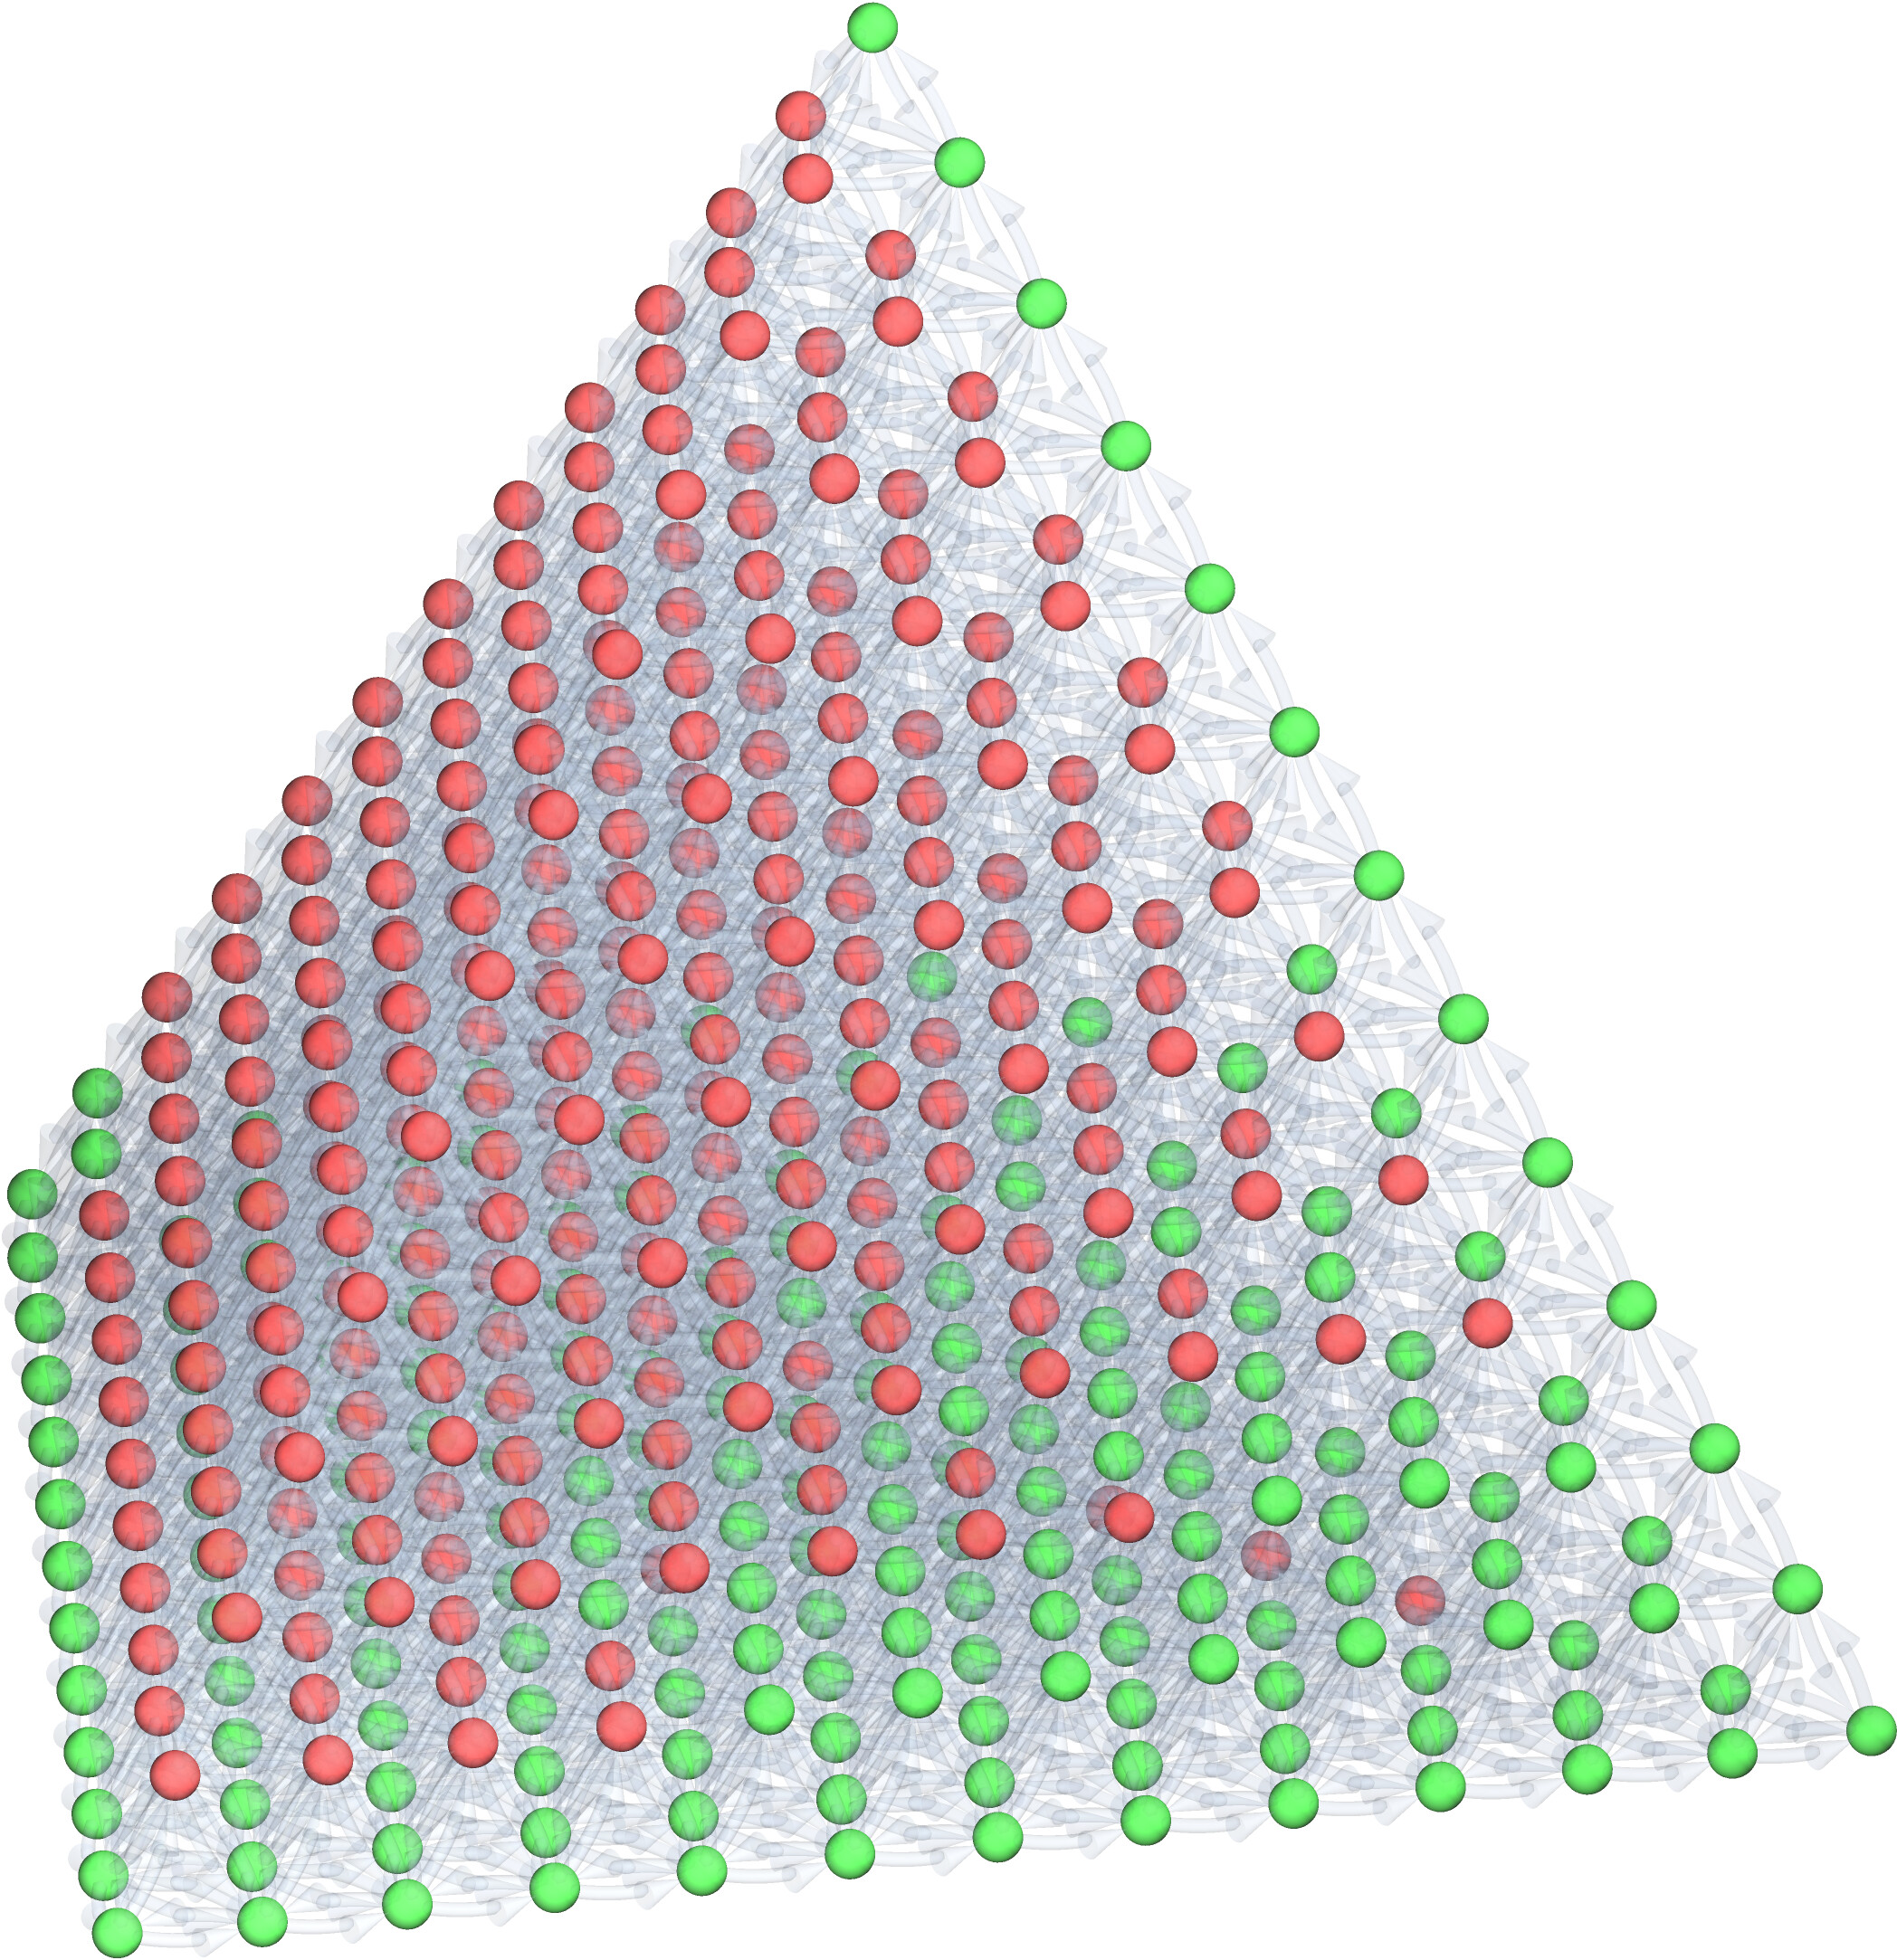
\includegraphics[width=0.7\textwidth]{infeasibilitygliding/InfeasibilityGliding_Full.jpeg}
    \caption{Feasibility map over compositional tetrahedron (3-simplex) formed by all combinations of Ti50 Zr50, Hf95 Ti5, Mo33 Nb33 Ta33, Mo80 Nb10 W10 discretized at 12 divisions per dimension. The positions in the 7-component elemental space obtained from \texttt{nimplex}, described in Chapter \ref{chap:nimplex}, were used to run \texttt{pycalphad} \cite{Otis2017Pycalphad:Python} evaluations and constrained by limiting phases present at equilibrium at 1000K to single or many solid solution phases. Roughly half of the compositions are infeasible, with most of them forming a single large region.}
    \label{infeasibilitygliding:fig:fullcomputation}
\end{figure}

\section{Gliding on the Boundaries of Infeasibility} \label{infglide:sec:glide}

As shown in Figure~\ref{infeasibilitygliding:fig:fullcomputation}, the infeasible region of space is generally continuously bounded by a single smooth surface, with only a few other small infeasible points. Thus, in principle, the infeasible space could be efficiently navigated around through only surface point calculations, without considering the bulk of internal points that cannot be accessed, accomplishing the goals set in Section~\ref{infglide:sec:intro}. This work coins the term \emph{Infeasibility Gliding} to describe such an approach.

\subsection{Underlying Assumptions} \label{infglide:ssec:assumptions}

One core assumption that needs to be considered in exploration based on the infeasibility gliding is that the high-dimensional surface bounding the infeasible space is highly smooth, or in terms of phase stability, that the region where a given infeasible phase exists (often spanning multiple phase regions) is smoothly bound. While not possible to be proven to be valid in every system, it can be shown to be reasonable for exploration problems, as it (1) is \emph{not required} for the method to glide around the boundary, but only to argue for low computational cost, and (2) it is generally true for metallic systems of interest, as depicted in an example in Figure~\ref{infeasibilitygliding:fig:katesphasemap} from \citet{Elder2023ComputationalValidation}, as well as many other studies, like ones by \citet{Bobbio2022DesignCompositions}, \citet{Sun2024MaterialsMap:Ag-Al-Cu}, \citet{Gao2016SenaryHfNbTaTiVZr}, or \citet{Zhao2014ExperimentalSystem}.

\begin{figure}[H]
    \centering
    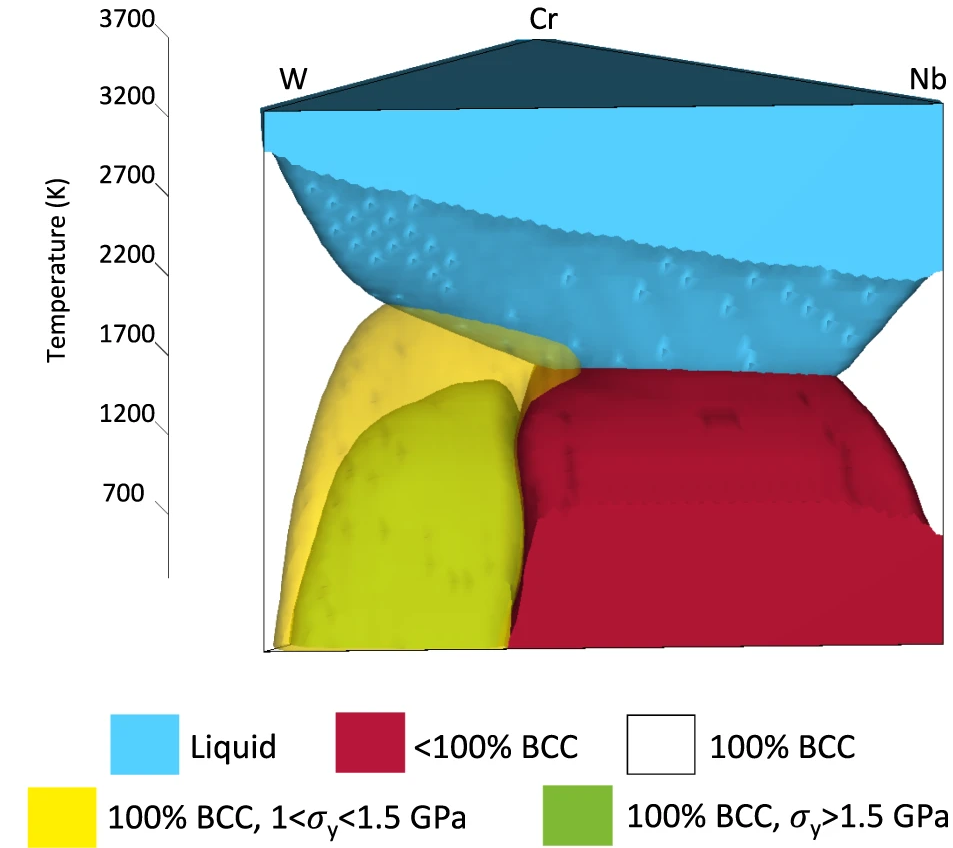
\includegraphics[width=0.5\textwidth]{infeasibilitygliding/PhaseTernaryMap_Elder2023.png}
    \caption{A view of ternary Cr-Nb-W phase diagram projected across a temperature range of phase classes, further augmented by imposing predicted property value constraints. It depicts the smoothness of the infeasible region boundary (red) and the increasingly smooth boundary of the property-constrained region. Taken from Figure 2b in \citet{Elder2023ComputationalValidation} under CC BY 4.0 license.}
    \label{infeasibilitygliding:fig:katesphasemap}
\end{figure}


\subsection{Unbiased Exploration Searches} \label{infglide:ssec:unbiasedexplore}

With the infeasibility gliding approach, one can now perform the same traversal over a graph as done in Section~\ref{infglide:sec:exploitgraph}; however, it is limited to exploring only the neighborhood of the feasible points and, thus, not going into the inside of the infeasible region. This highly desirable behavior, reducing computation by a factor of roughly 2, is shown in Figure~\ref{infglide:sec:glide}, in contrast to the earlier Figure~\ref{infeasibilitygliding:fig:fullcomputation}. The presented results are taken from the second \texttt{nimplex} workshop, which has been adapted as Appendix~\ref{chap:nimplextutorial2} and can be consulted for step-by-step details of an example implementation.

\begin{figure}[H]
    \centering
    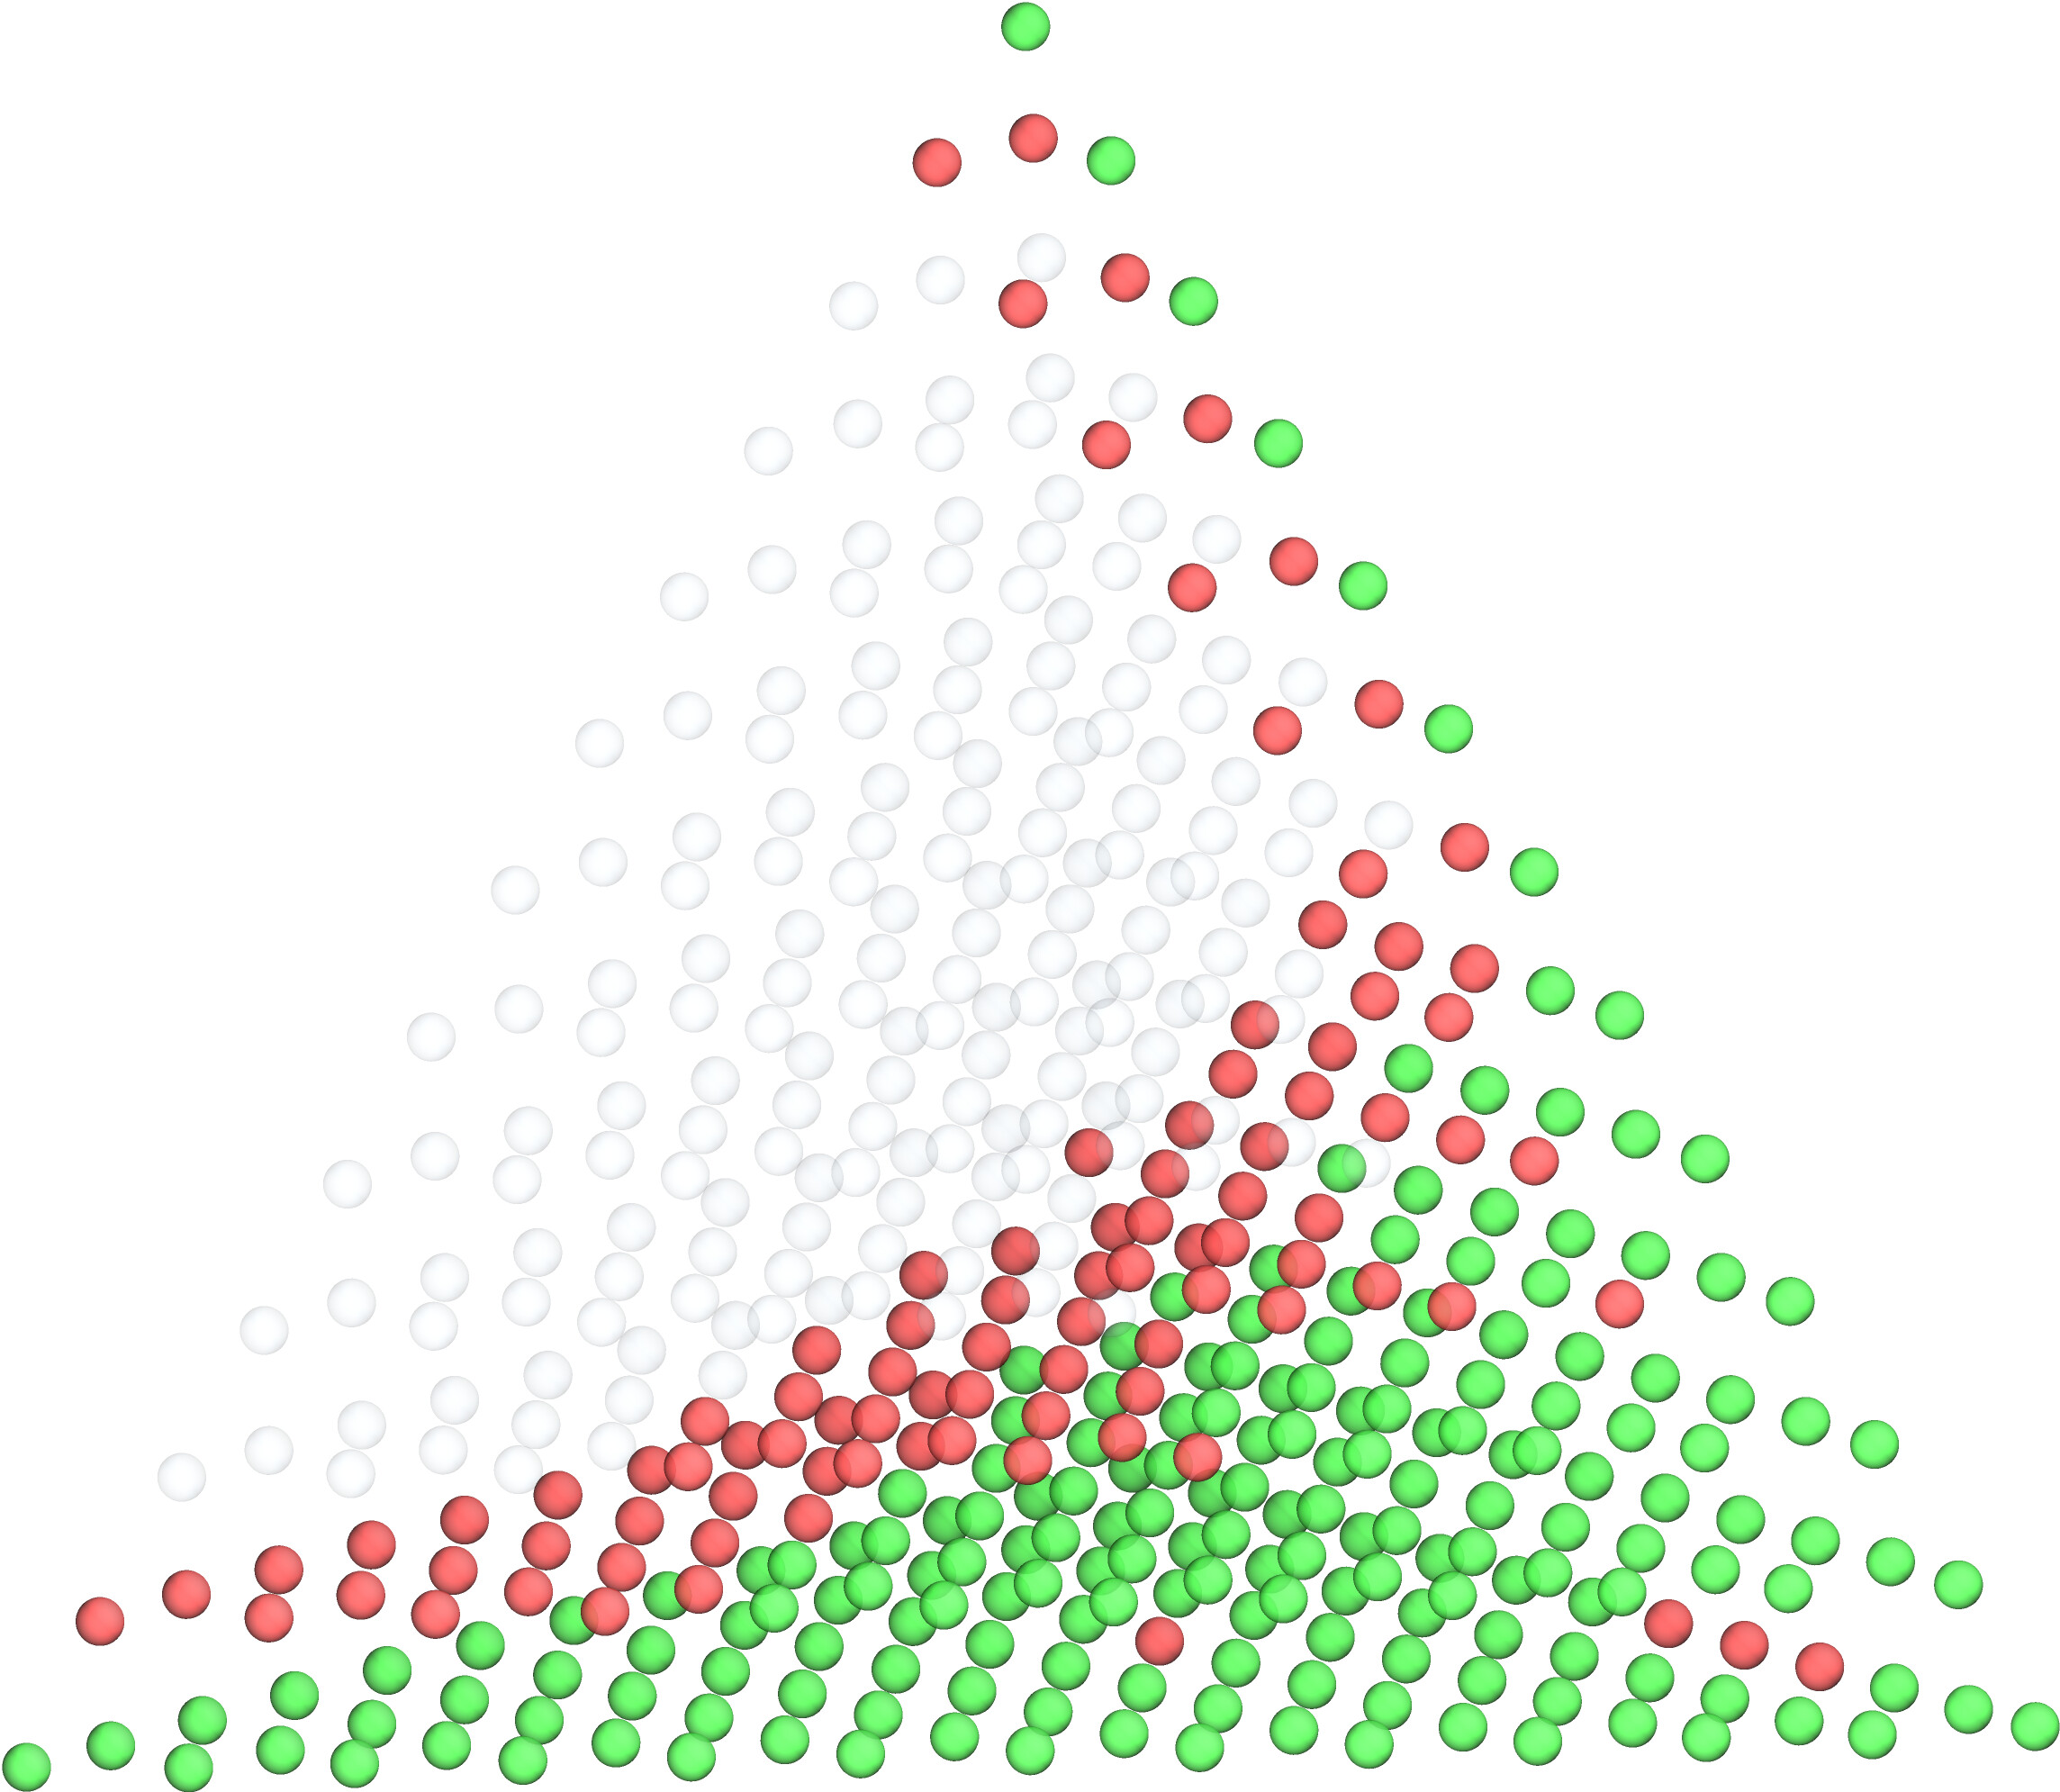
\includegraphics[width=0.7\textwidth]{infeasibilitygliding/InfeasibilityGliding_Glide.jpeg}
    \caption{The same problem as in Figure \ref{infeasibilitygliding:fig:fullcomputation} solved by iteratively exploring all feasible paths in the compositional graph in a depth-first approach, which can be started from one or multiple points, and terminated once the goal is reached or once all of the feasible space is explored.}
    \label{infeasibilitygliding:fig:glide}
\end{figure}


\printbibliography[heading=subbibintoc]